% ------------------------------------------------------------------------------
% Metodologia
% ------------------------------------------------------------------------------

\chapter{Metodologia}\label{chap:metodologia}

{\color{red} Para o TCC2, eu preciso que você reescreva o capítulo mudando o tempo verbal do futuro para o presente ou passado. Ou seja, ao invés de dizer que irá fazer algo, preciso que você escreva que está propondo tal coisa e que tal coisa foi feita da forma X.}

Como fundamento do desenvolvimento desse trabalho, está a utilização das 
técnicas de ES para tornar o dia-a-dia de trabalho e gestão de 
atividades mais claros e concisos. Além disso, serão especificadas deficiências no 
processo ou ciclo de vida que, apesar de já serem conhecidas, não estão bem 
colocadas ou esclarecidas. 

Pode ser definido como primeira etapa de trabalho a definição do ciclo de vida como 
é hoje. Através do estudo do fluxo atual, são definidos os eventos de cada estágio, 
os entregáveis de cada estágio e os pontos de decisão entre os 
estágios. 

Recapitulando, o serviço prestado é basicamente a concepção de diferentes 
sistemas para atender requisitos específicos em cada caso trazido ao nosso {\color{red}(geralmente, não é colocado em primeira pessoa; você pode escrever como se fosse um observador de fora, mesmo sendo parte da coisa)} time, 
para desenvolvimento e/ou sustentação.   

Para ajudar a construir esse ciclo de vida será desenvolvida a arquitetura dos 
elementos do sistema e estabelecida a relação com as funcionalidades. Assim, pode 
ser definido todas as opções de possíveis sistemas do serviço prestado, através das 
combinações de elementos do sistema e das funcionalidades. 

Após essa primeira parte do trabalho, com os artefatos e documentações já 
produzidas, será feita a análise e listagem, dos problemas e deficiências 
encontradas agora. Focado na parte de gestão de requisitos e rastreabilidade dos 
sistemas desenvolvidos, serão dados mais detalhes e especificações dos problemas 
identificados bem como apresentada uma proposta de solução. 

Sobre a proposta mencionada anteriormente, se trata do desenvolvimento de uma 
aplicação \textit{low code} utilizando as ferramentas e recursos da \textit{Power Platform} para 
correlacionar os elementos do sistema e os requisitos levantados. 

Depois de desenvolvida a aplicação, ela será colocada em operação para a coleta 
de dados de utilização, bem como a percepção dos outros integrantes do time sobre 
pontos de melhoria ou críticas sobre ela. Métricas de estimação de esforço de novas 
funcionalidades ou alterações podem ser coletadas com mais precisão após essa 
implementação, pois as relações entre os componentes estão definidas com 
clareza. Esse resultado poderá ser coletado com uma comparação entre as 
estimativas para uma mesma tarefa utilizando ou não a ferramenta desenvolvida. 

Por fim, será concatenados todos os resultados colhidos para uma análise e 
avaliação do trabalho realizado. Pontos de melhoria notados no decorrer das 
atividades realizadas, mas fora do escopo definido, serão indicados para futuras 
evoluções ou prosseguimento do trabalho. 

	

	\section{{\color{blue}Ciclo de vida}}

	Inicialmente definiu-se em formato de fluxograma o processo do serviço prestado, para dessa forma ser 
	mais fácil o entendimento da ordem das etapas. Depois traremos essa representação para o formato esperado
	na ES. A figura \ref{fig:metodologia:processFlow} mostra esse fluxograma.
	
	\begin{figure}[h]
		\centering
		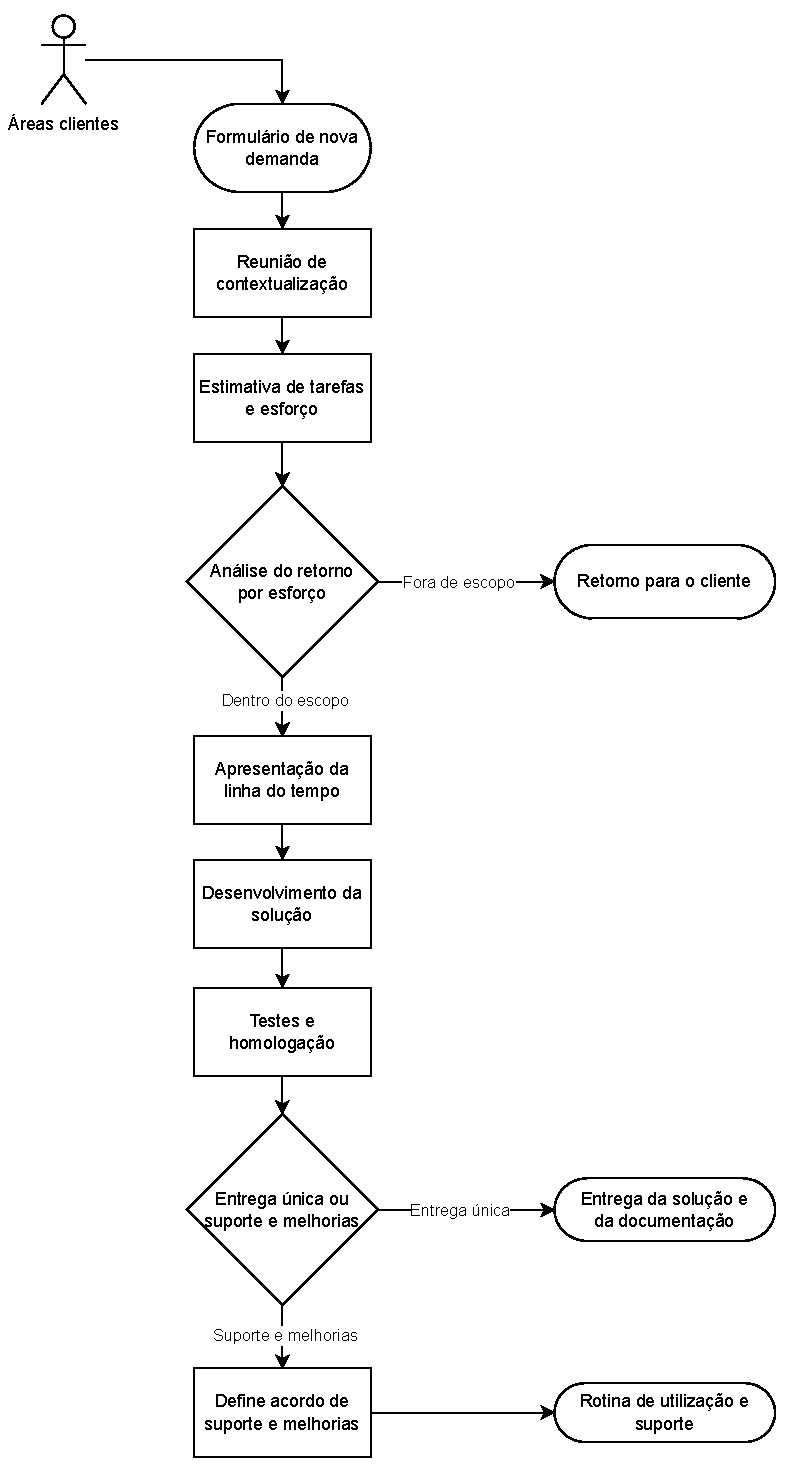
\includegraphics[width=0.6\textwidth]{./figuras/processFlow.pdf}
		\caption{Fluxograma do processo que descreve o serviço prestado.}
		\label{fig:metodologia:processFlow}
	\end{figure}
	
	Entrando agora no detalhamento de cada um dos blocos existentes:
	\begin{itemize}
		\item \textbf{Formulário de novo desenvolvimento}
		\begin{itemize}
			\item Descrição: Esse formulário é o ponto de entrada de uma nova demanda para o time. Quando uma área
			cliente manifesta a necessidade e procura o auxílio do time, ela é direcionada a responder esse formulário
			online com uma série de perguntas. E há ainda, casos em que auditorias internas encontram irregularidades em processos existentes,
			e os encaminham para entrar em contato com o time para possíveis soluções de remediação, novamente eles são direcionados para responder o formulário.
			\item Objetivos: Obter informações de contato e departamento do requisitante bem como o centro de custo em caso de
			possíveis cobranças no futuro. Levantar informações iniciais sobre a solução desejada como classificação dos dados envolvidos, 
			interdependência com outras áreas e quais dores seriam sanadas com o desenvolvimento.
			Coletar dados e percepções que ajudem a mensurar o valor para a área e para a empresa como um todo, ao ser desenvolvida uma
			solução para essa demanda. Solicitar documentação disponível do processo atual caso exista.
			\item Saídas: Registro das respostas ao formulário, anexos e documentações enviadas.
		\end{itemize}
		\item \textbf{Reunião de contextualização}
		\begin{itemize}
			\item Descrição: Após recebida e revisada a resposta do formulário, o gerente de projetos organiza essa reunião com os desenvolvedores
			envolvidos e o requisitante, orientando-o a convidar todas as outras partes interessadas. Nessa reunião, o requisitante faz uma nova explicação dos problemas e possíveis
			de soluções, e também são sanadas possíveis dúvidas sobre as respostas do fomulário e sobre a documentação enviadas anteriormente.
			\item Objetivos: Entender o papel de todas as partes interessadas na operação. Ver o processo atual existente sendo executado integralmente
			pelos responsáveis. Obter exemplos de artefatos do processo como emails enviados, arquivos gerados ou compartilhados,
			indicadores calculados e outros artefatos que sejam importantes, caso existam. Discutir casos de uso e cenários que não existem atualmente
			mas são desejáveis na solução. Discutir políticas de retenção de dados.
			\item Saídas: Gravação da reunião e operação atual. Arquivos com os exemplos de artefatos do processo atual.
		\end{itemize}
		\item \textbf{Estimativa de tarefas e esforço}
		\begin{itemize}
			\item Descrição: Nessa etapa os desenvolvedores de maior senioridade realizam uma sintetização das necessidades e requisitos para propor
			um ou mais cenários de solução. Assim, em um curto espaço de tempo, são definas histórias de usuário em um alto nível, sem muito detalhamento,
			para que seja estimado o esforço e tempo total necessário para o desenvolvimento dos cenários de solução. 
			\item Objetivos: Definir cenários de solução para o caso trazido pelo cliente. Estimar o esforço e tempo necessário para executar as tarefas definidas para cenário.
			\item Saídas: Documento com cenários propostos, tempo e esforço necessários para cada um. 
		\end{itemize}
		\item \textbf{Análise do retorno por esforço}
		\begin{itemize}
			\item Descrição: Ao receber o documento da etapa anterior o gerente de projetos de reúne com o gerente e o diretor da área,
			onde realizam uma análise de enquadramento de escopo de todas as submissões que estão aguardando o início do desenvolvimento, e 
			depois uma priorização das que serão iniciadas. Essa etapa é realizada em uma menor frenquência,
			geralmente bimestralmente, salvo exceções em que envolvem uma falha em auditoria e que precisam de mais celeridade.
			\item Objetivos: Definir se a demanda solicitada está no escopo do time (dentro das capacidades técnicas do time, dentro do tempo máximo de desenvolvimento por projeto, não conter
			dados estritamente confidenciais, gerar um valor que valha o investimento). Priorizar a ordem de execução das tarefas.
			\item Saídas: Lista com os projetos selecionados e priorizados para execução.
		\end{itemize}
		\item \textbf{Retorno para o cliente}
		\begin{itemize}
			\item Descrição: Quando um projeto é definido como fora de escopo, é marcada uma reunião com o requisitante e apresentado 
			os motivos da decisão. A depender do motivos são passadas orientações para a área cliente, como procurar outro time de desenvolvimento interno na empresa,
			utilizar uma ferramenta existente no mercado, contratar time externo para executar o projeto, ou mesmo redefinir os requisitos e necessidades e submeter novamente para análise.
			Essa etapa é um dos possíveis fins do fluxo de serviço.
			\item Objetivos: Apresentar uma devolutiva ao requisitante da demanda. Orientar sobre possíveis alternativas.
			\item Saídas: Ata da reunião com principais tópicos, decisões, e participantes.
		\end{itemize}
		\item \textbf{Apresentação da linha do tempo do projeto para o cliente}
		\begin{itemize}
			\item Descrição: Quando um projeto é definido como dentro do escopo e priorizado, é marcada uma reunião com o requisitante
			para dar um retorno sobre essa priorização. O gerente de projetos apresenta como ficou a linha do tempo estimada para os diferentes cenários e quando será
			iniciado o desenvolvimento.
			\item Objetivos: Apresentar o cronograma e início do desenvolvimento. Definição de qual cenário será desenvolvido. Coletar possíveis ressalvas quanto aos prazos informados.
			Definir agendas para acompanhamento do progresso do desenvolvimento.
			\item Saídas: Ata da reunião com principais tópicos, decisões, e participantes. Agenda com as reuniões de acompanhamento.
		\end{itemize}
		\item \textbf{Desenvolvimento da solução}
		\begin{itemize}
			\item Descrição: Esta é a etapa dedicada ao trabalho de desenvolvimento de programação da solução proposta e escolhida. A partir das histórias de usuário
			criadas anteriormente, semanalmente são criadas taferas detalhando as atividades a serem realizadas na próxima semana para cada história de usuário.
			\item Objetivos: Detalhar as histórias de usuário em tarefas. Executar as tarefas de cada história de usuário.
			\item Saídas: Solução desenvolvida com todas as suas fucionalidades.
		\end{itemize}
		\item \textbf{Teste e homologação}
		\begin{itemize}
			\item Descrição: Ao ser finalizado o desenvolvimento da solução é realizada um demonstração ao requisitante e às partes interessadas.
			A solução é implantada no ambiente de qualidade para que os usuários façam testes e validem se as funcionalidades e requisitos foram cumpridos.
			Em paralelo o time de desenvolvimento trabalha para corrigir problemas encontrados.
			\item Objetivos: Usuários validarem as funcionalidades da solução desenvolvida. Corrigir possíveis problemas encontrados. Definir uma data para fim dos testes em qualidade. 
			\item Saídas: Relatório de problemas encontrados na ferramenta. Relatório com possíveis melhorias futuras. Relatório com as correções realizadas.
		\end{itemize}
		\item \textbf{Entrega única ou suporte e melhorias}
		\begin{itemize}
			\item Descrição: Nessa etapa se inicia o encerramento do projeto. É realizada uma reunião com o requisitante e as partes interessadas, onde discute-se
			sobre como foi o andamento do projeto e são explicadas as opções de continuidade para a área cliente demandante. Onde existem as opções de contratarem 
			um plano de suporte e melhorias com o time de desenvolvimento ou seguirem por conta própria com a solução desenvolvida. 
			\item Objetivos: Formalizar a entrega da solução desenvolvida. Apresentar com mais detalhes as opções de continuidade. Estipular um prazo para retorno sobre qual será a opção escolhida, caso não seja decidido na reunião.
			\item Saídas: E-mail com a formalização da entrega. Prazo para decisão dos próximos passos.
		\end{itemize}
		\item \textbf{Envio do pacote da solução e entrega da documentação}
		\begin{itemize}
			\item Descrição: Caso o requisitante e sua área decidam por não contratar o pacote de suporte e melhorias, são enviadas por e-mail as intruções de como dar continuidade à operação da solução, bem como o pacote contendo a própria solução desenvolvida. Espera-se um atestado de recebimento or parte do requisitante.
			\item Objetivos: Enviar documentação fucional da solução desenvolvida. Enviar pacote com a solução desenvolvida.
			\item Saídas: E-mail com os documentos de entrega do projeto. Atestado de recebimento dos arquivos, que simboliza o encerramento do projeto.
		\end{itemize}
		\item \textbf{Acordo de suporte e melhorias}
		\begin{itemize}
			\item Descrição: Ao optar por seguir com o pacote de suporte e melhorias, são definidas as horas mensais dedicadas e valor a ser pago para esse pacote. Além disso, é demonstrado como são abertas requisições de suporte e melhorias.
			\item Objetivos: Definir horas e custos mensais do pacote se suporte e melhorias. Obter autorização para débito no centro de custo da área cliente.
			\item Saídas: E-mail com acordo de suporte e melhorias.
		\end{itemize}
		\item \textbf{Rotina de manutenção e suporte}
		\begin{itemize}
			\item Descrição: A aplicação é implantada no ambiente produtivo e liberada para operação aos usuários.
			\item Objetivos: Implantar a solução em produção. Encerrar o projeto de desenvolvimento. Iniciar suporte e manutenção da solução.
			\item Saídas: E-mail com intruções de acesso e utilização da ferramenta. E-mail com as instruções para criação de requisições de suporte.
		\end{itemize}
	\end{itemize}

	Para as áreas que não optaram por seguir com um acordo de suporte e melhorias, caso seja necessário uma nova implementação ou modificação relacionada à soluçao desenvolvida, deverão responder novamente o formulário e passar por todo o processo de análise de retorno por investimento e priorização, como uma nova demanda.
	Já as que tem o acordo de suporte e melhorias, podem utilizar as horas mensais e fazer o balanceamento das mesmas para realizar essas implementações sem passar por todo o processo. Entretanto, mesmo com o acordo, caso seja uma modificação muito grande ou uma nova funcionalidade que demande muito tempo de desenvolvimento, é necessário responder o formulário e iniciar como uma nova demanda ao time, porém ao fim não precisam de um novo acordo de suporte e melhorias, pois já o possuem.

	Trazendo o cilo de vida em ``V'' mencionado anteriormente, as areas que possuem o contrato de suporte percorrem todas os estágios, dos dois lados do ``V''. Já as outras áreas,
	param na primeira metade.

	\subsection{{\color{blue}Adequação de representação}}

	Tendo todas as etapas do processo sido explicadas, são feitas sua relações com os estágios e fases do ciclo de vida proposto na engenharia de sistemas.
	De maneira descritiva sem ainda avaliar a otimização ou melhoria do ciclo de vida podemos representar o ciclo de vida com as figuras \ref{fig:metodologia:currentConceptPhases}, \ref{fig:metodologia:currentDevelopmentPhases} e \ref{fig:metodologia:currentPostDevelopmentPhases}.
	
	\begin{figure}[h]
		\centering
		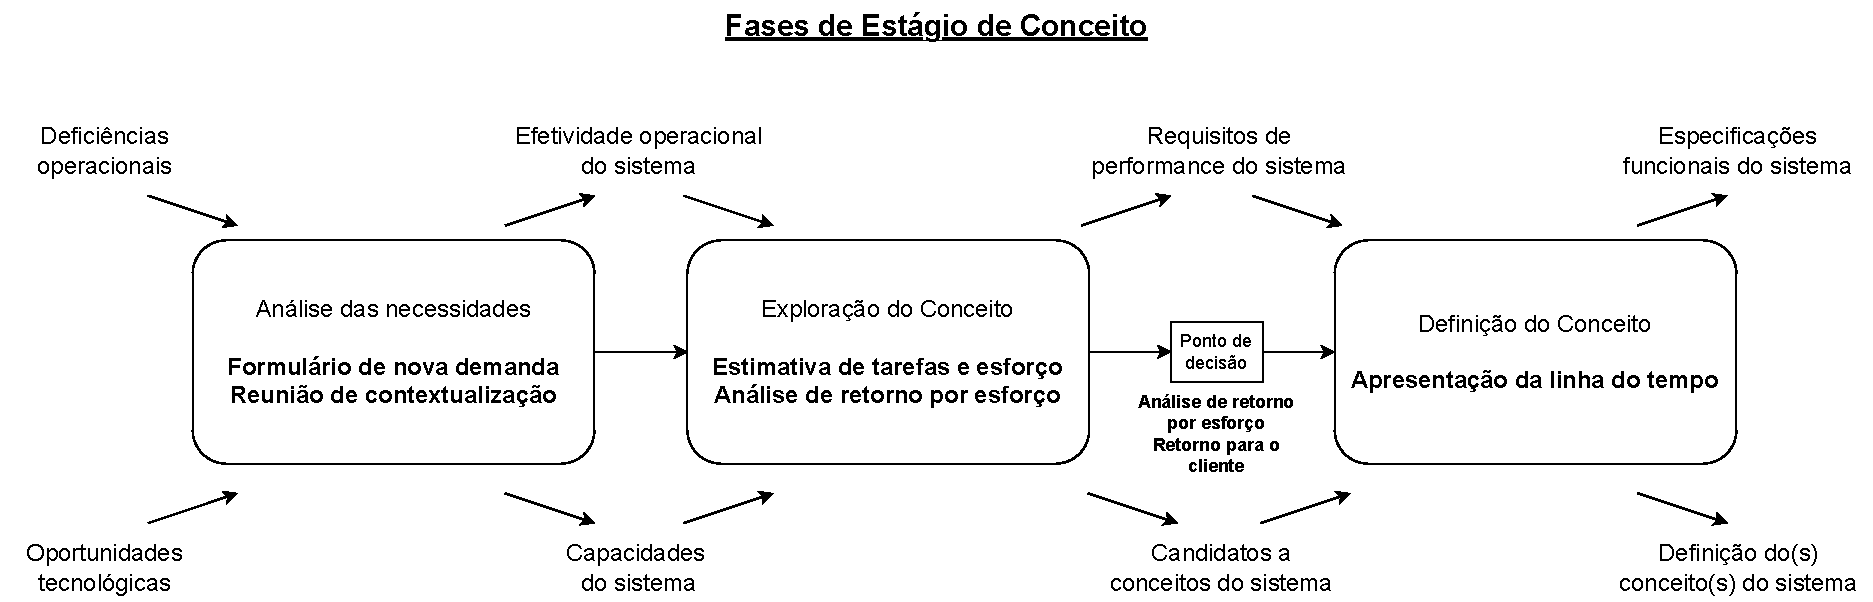
\includegraphics[width=\textwidth]{./figuras/currentConceptPhases.pdf}
		\caption{Relação com as fases do estágio de Conceito}
		\label{fig:metodologia:currentConceptPhases}
	\end{figure}

	Olhando para o estágio de Conceito na figura \ref{fig:metodologia:currentConceptPhases}, na fase de \textbf{Análise das necessidades} temos as etapas
	de \textbf{Fomulário de nova demanda} e \textbf{Reunião de contextualização}. De fato, nessas etapas é realizado o primeiro contato com as áreas 
	clientes e visto a operação que se deseja digitalizar ou otimizar. De forma macro já é entendida as principais capacidades do sistema bem como uma pré-análise de quais tecnologias utilizar.

	Agora na fase de \textbf{Exploração do Conceito} foram alocadas as etapas de \textbf{Estimativa de tarefas e esforço} e \textbf{Análise de retorno por esforço}. A etapa de
	\textbf{Estimativa de tarefas e esforço} já começa a documentar alguns requisitos e separar subsistemas para mensuração de esforço de desenvolvimento, nela são propostas mais de uma abordagem
	de solução quando aplicável e também é analisada a viabilidade técnica. A etapa de \textbf{Análise de retorno por esforço} também
	foi posicionada nessa fase pois nela ocorre a análise de viabilidade estratégica de desenvolvimento do sistema.

	Foi destacado ainda o ponto de decisão entre a fase de \textbf{Exploração do Conceito} e de \textbf{Definição do Conceito}, que é justamente após a análise de viabilidade
	estratégica. Nesse ponto, é decidido se será empenhado mais esforço a fim de continuar o trabalho para o desenvolvimento da solução ou o cancelamento da iniciativa, interrompendo o ciclo
	de vida de avançar, acontece nesse caso a etapa de \textbf{Retorno ao Cliente}.

	Na fase de \textbf{Definição do Conceito} temos a etapa de \textbf{Apresentação da linha do tempo}, pois nessas apresentação são sugeridas as alternativas de desenvolvimento que satisfaçam
	os requisitos estabelecidos, de maneira integral ou não, e suas justificativas para serem utilizadas.
	
	\begin{figure}[h]
		\centering
		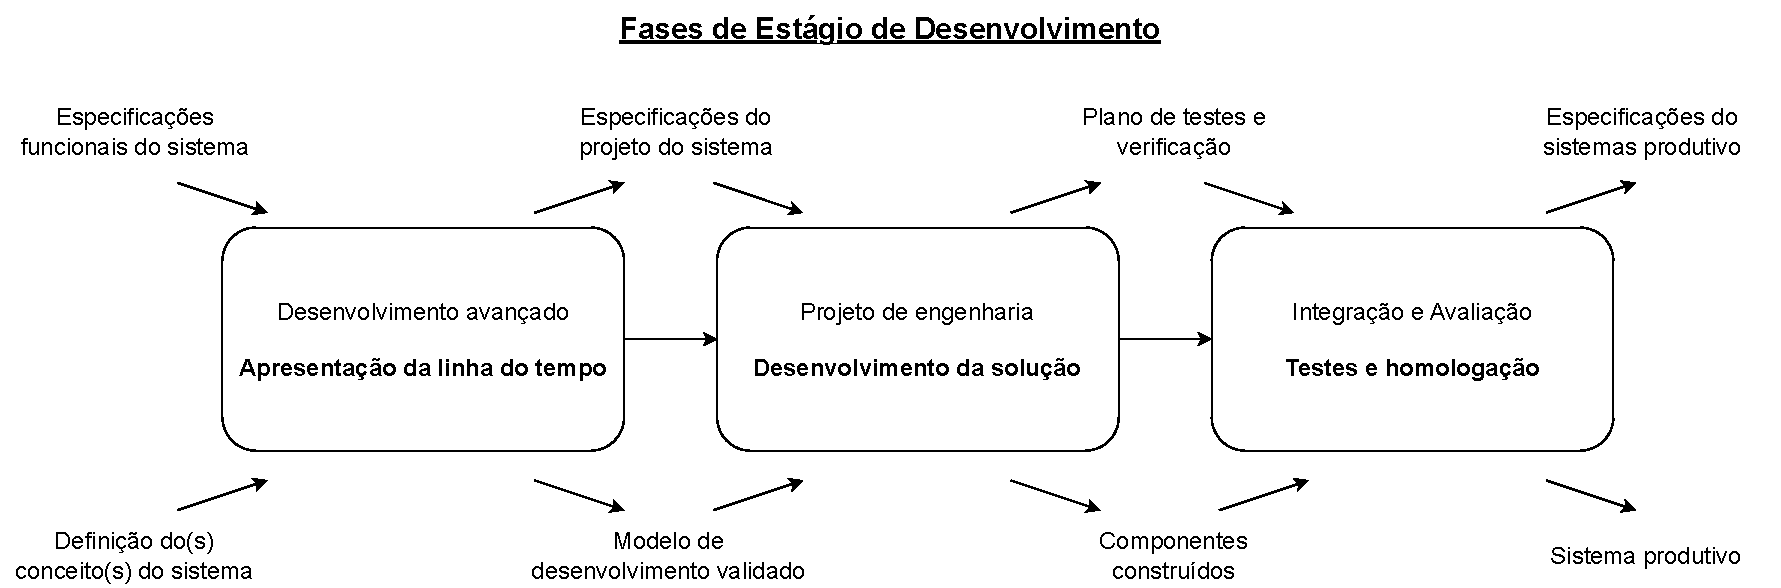
\includegraphics[width=\textwidth]{./figuras/currentDevelopmentPhases.pdf}
		\caption{Relação com as fases do estágio de Desenvolvimento}
		\label{fig:metodologia:currentDevelopmentPhases}
	\end{figure}

	Voltando a atenção para o estágio de Desenvolvimento, na primeira fase de \textbf{Desenvolvimento Avançado} temos novamente a etapa de \textbf{Apresentação da linha do tempo}, pois é realizada
	a apresentação das histórias de usuário, buscando a validação das partes interessadas. São apresentadas as principais funcionalidades junto com a programação de desenvolvimento e também discutido
	o cronograma, captando os riscos do mesmo, no ponto de vista dos outros interessados.

	Na fase de \textbf{Projeto de Engenharia} se encontra a etapa de \textbf{Desenvolvimento da solução}, é feita a programação dos componentes do sistema através das histórias de usuário definidas semanalmente.
	Nesse caso os desenvolvedores e engenheiros empenham os esforços nos componentes onde são especialistas, e depois de desenvolvidos os testam individualmente.

	Por fim, na fase de \textbf{Integração e avaliação} está alocada a etapa de \textbf{Testes e Homologação} visto nessa etapa é realizada a integrações entre os componentes e os testes juntamente com a
	área demandante e um grupo pequeno do time operacional para simular o dia a dia de utilização da solução. São avaliadas a qualidade e completude das
	funcionalidades pré-estabelecidas anteriomente, e uma avaliação geral do escopo do sistema.

	\begin{figure}[h]
		\centering
		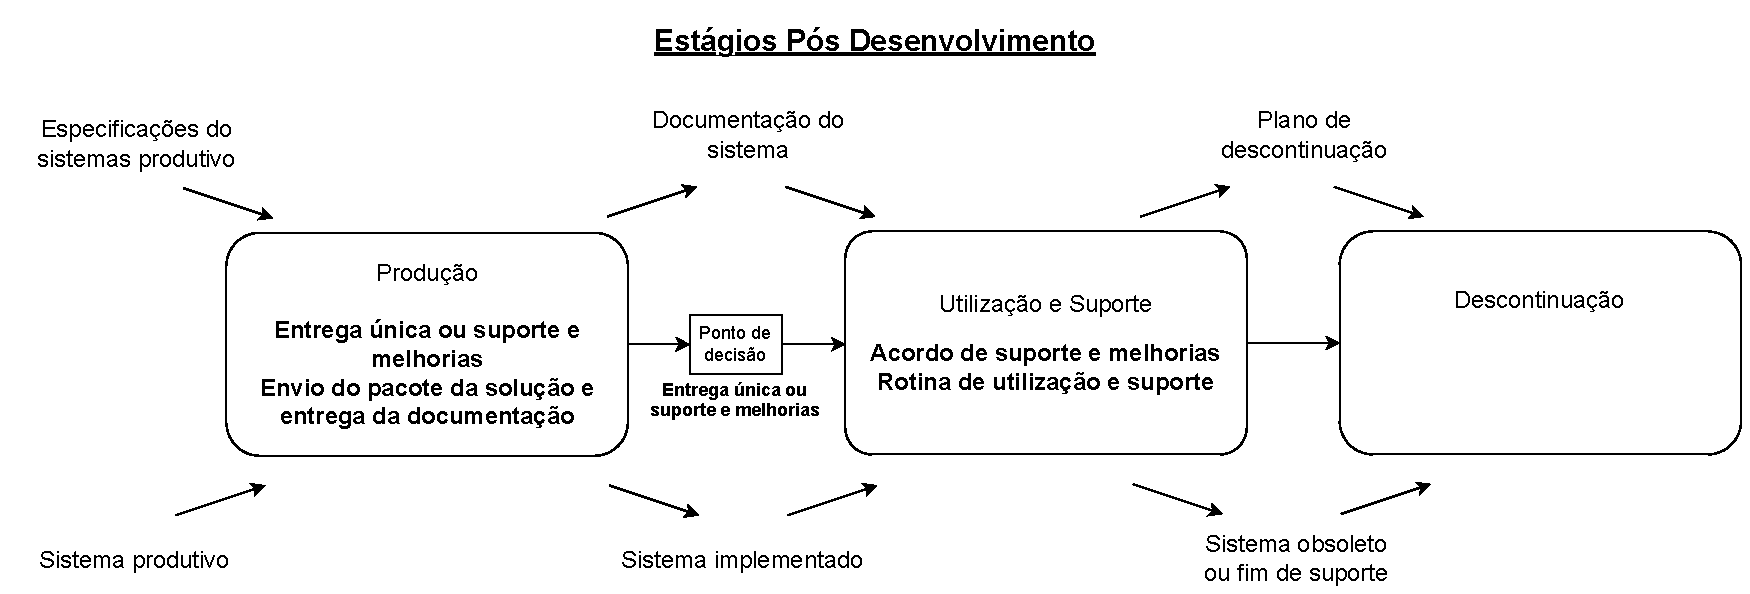
\includegraphics[width=\textwidth]{./figuras/currentPostDevelopment.pdf}
		\caption{Relação com os estágios Pós-Desenvolvimento}
		\label{fig:metodologia:currentPostDevelopmentPhases}
	\end{figure}

	Nos estágios de pós-desenvolvimento, em \textbf{Produção} temos as etapas de \textbf{Entrega única ou suporte e melhorias} e \textbf{Envio do pacote da solução e entrega da documentação},
	na primeira ocorre o aceite da entrega da solução/sistema e após isso é realizado a implantação do sistema em ambiente produtivo.
	Nesse ponto a documentação do sistema também deve estar feita e disponibilizada. Uma nuance do estágio de produção ocorre de acordo com a decisão tomada pela area cliente na etapa \textbf{Entrega única ou suporte e melhorias}, pois caso não optem
	pelo plano de suporte e melhoria, a implantação do sistema ocorre em um ambiente gerenciado por eles, e não pelo time de desenvolvimento, e por isso ocorre a etapa \textbf{Envio do pacote da solução e entrega da documentação}.

	É destacado outro ponto de decisão, entre o estágio de \textbf{Produção} e o de \textbf{Utilização e Suporte}, pois como dito, o ciclo de vida continua apenas se for feito a contração do serviço de suporte.
	Ressaltando que o sistema vai ser utilizado, mas deixa de ser responsabilidade do time de desenvolvimento.

	O estágio de \textbf{Utilização e Suporte} compreende as etapas de \textbf{Acordo de suporte e melhorias} e \textbf{Rotina de utilização e suporte}, onde os usuários, já utilizando o sistema, relatam falhas, problemas e melhorias que são corrigidas
	ou implementas ainda nesse estágio, ou seja, a segunda metade do ciclo de vida em ``V''.

	Ainda não existe uma etapa criada para \textbf{Descontinuação}, sendo que o time é relativamente novo com cerca de dois anos de criação
	não houve caso de obsolescência mapeado até então.

	\subsection{{\color{blue}Avaliação do ciclo de vida}}

	Ao longo da repetição desse ciclo de vida para cada solução desenvolvida, já havia sido notado um deficiência
	na parte de definição e validação de conceito. Por vezes, já no fim da fase de \textbf{Projeto de Engenharia} ou durante a fase de \textbf{Integração e avaliação}
	eram identificadas funcionalidades essenciais que não havia sido mapeadas, ou ainda um desenvolviemento que tecnicamente funcionava mas que desenpanhava uma 
	funcionalidade desalinhada com a real intenção das partes interessadas.

	Olhando para a representação do ciclo de vida de acordo com as definições da ES, fica mais claro identificar a raiz dessa deficiência bem como o que
	pode ser feito para mudar. A transição entre os estágios de Conceito e Desenvolviemento, marcado pelas fases de Definição de Conceito e Desenvolvimento avançado, apresenta
	uma falta de artefatos ou documentos que permitiriam essa transição de forma suave mas concisa.

	Um ponto em destaque é que no caso essas duas fases estão representadas por uma única etapa, e que não contempla todas as características das fases, a etapa
	de \textbf{Apresentação da linha do tempo}. Ela comtempla características como a definição e validação do conceito do sistema, mas não desce mais níveis na hierarquia,
	como validação de subsistemas ou alocação de componentes.

	Olhando em conjunto para a tabela \ref{tab:revisao:systemMaterialization} sobre a materialização do sistema e as fases de Definição de Conceito e Desenvolvimento avançado,
	é observado e destacado em vermelho e laranja os seguintes pontos falhos, mostrados na figura \ref{fig:metodologia:lifeCycleIssues}.

	\begin{figure}[h]
		\centering
		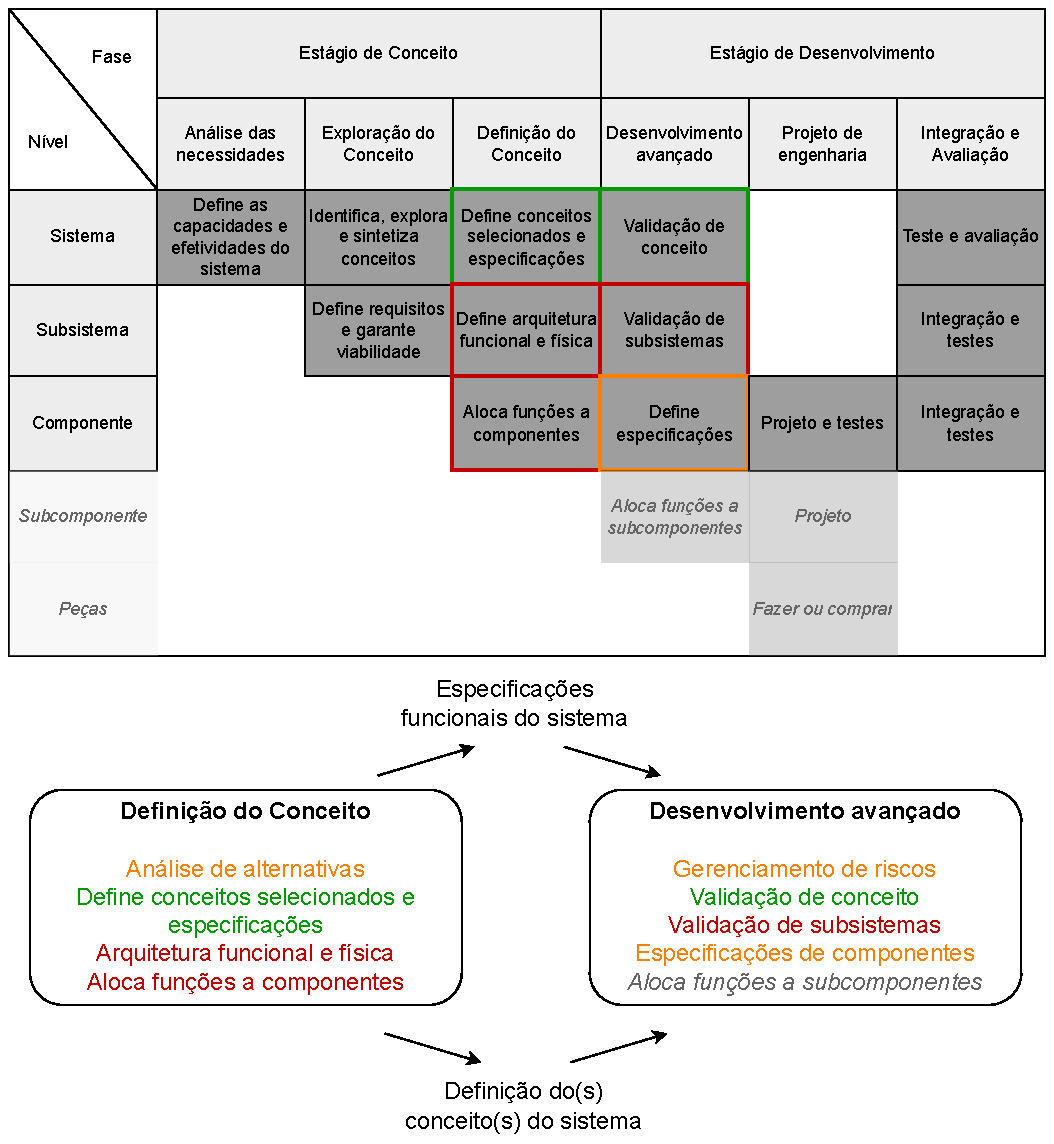
\includegraphics[width=0.8\textwidth]{./figuras/lifeCycleIssues.pdf}
		\caption{Destaque dos pontos falhos no ciclo de vida}
		\label{fig:metodologia:lifeCycleIssues}
	\end{figure}

	Em vermelho, temos as tarefas ou atividades que são completamente ignoradas nessas fases:
	\begin{itemize}
		\item Arquitetura física e funcional: não é realizada a documentação da arquitetura do sistema na fase de definição de conceito, mesmo que os
		desenvolvedores já tenham uma boa noção de como seria o resultado final, sem esses artefatos não é possível a validação dos subsistemas, ou mesmo realizar um gerenciamento
		de riscos efetivo. Sem as arquiteturas definidas, mesmo que em auto nível, as outras partes interessadas não conseguem contribuir tanto no ponderamentos.
		\item Aloca funções a componentes: como não existe nenhuma das duas arquiteturas essa tarefa não é realizada, pois seria justamente definir as relacões entre as arquiteturas,
		e gerando assim uma forma de garantir a rastreabilidade do sistema.
		\item Validação de subsistemas: essa é outra tarefa que não é realizada justamente fela falta da documentação das arquiteturas do sistema. Sendo assim, é a raiz de algumas falhas de entendimento
		dos requisitos e que acarretam a inclusão ou modificação de funcionalidades no estágio de \textbf{Integração e avaliação}, e que afeta diretamente nos prazos estipulados.
	\end{itemize}

	Já em laranja, temos algumas atividades que são parcialmente realizadas no ciclo de vida atual:
	\begin{itemize}
		\item Análise de alternativas: Essa atividade é parcialemente realizada, pois 
		\item Gerenciamento de riscos:
		\item Especificações de componentes:
	\end{itemize}	




	\section{{\color{blue}Proposta de modificações}}
	
	\subsection{{\color{blue}Arquitetura do Sistema}}

	Na figura \ref{fig:metodologia:arquiteturaFisica} pode ser observada um padrão de arquitetura física para os sistemas desenvolvidos. Ela contém todos os possíveis
	elementos do sistema que podem ser utilizados para a arquitetura final de cada projeto executado. 
	\begin{figure}[h]
		\centering
		% \includegraphics[width=1\textwidth]{./figuras/lcurve.eps}
		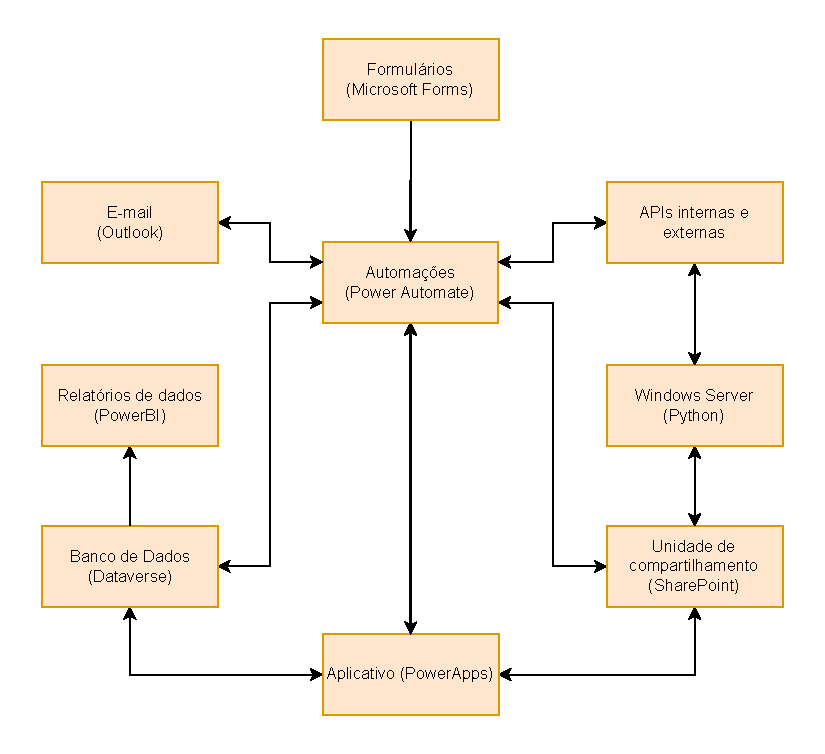
\includegraphics[width=1\textwidth]{./figuras/arquiteturaFisica.pdf}
		\caption{Padrão de arquitetura física dos sistemas desenvolvidos.}
		\label{fig:metodologia:arquiteturaFisica}
	\end{figure}

	Já na figura \ref{fig:metodologia:arquiteturaFuncional} temos o padrão de arquitetura funcional para os sistemas desenvolvidos, e mais uma vez, contém todas as possibilidades
	de funções disponíveis e que podem ser implementadas no sistema de interesse.
	\begin{figure}[h]
		\centering
		% \includegraphics[width=1\textwidth]{./figuras/scattering.eps}
		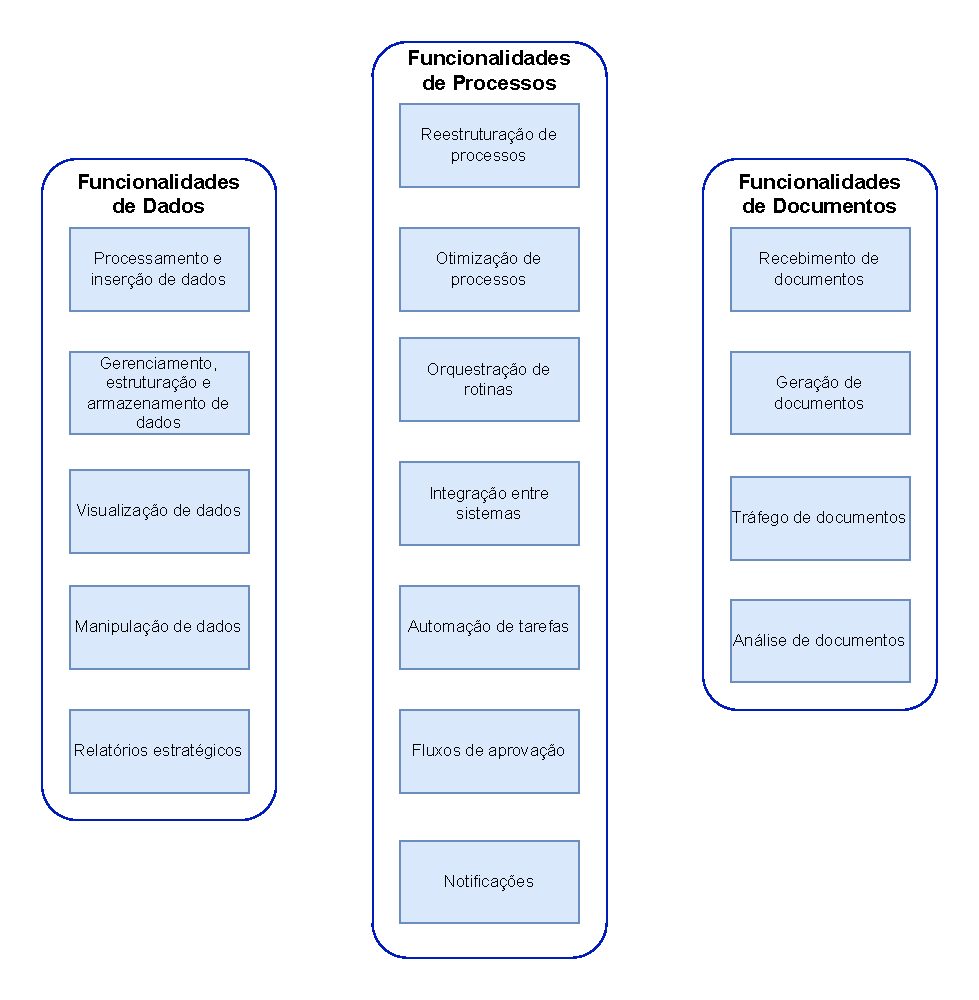
\includegraphics[width=1\textwidth]{./figuras/arquiteturaFuncional.pdf}
		\caption{Padrão de arquitetura funcional dos sistemas desenvolvidos.}
		\label{fig:metodologia:arquiteturaFuncional}
	\end{figure}


	\section{Instrumentos e Materiais}

	A documentação do ciclo de vida atual do sistema de serviço será feita a partir do desenvolvimento de diagrams que representarão os estágios e etapas do ciclo de vida do serviço prestado. Nelas serão destacas as saídas e entradas. O diagrama será confeccionado na ferramenta online \textit{Draw.io}, 
	que é uma ferramenta gratuita para o desenho de diagramas de diferentes 
	tipos e não restringe o salvamento do arquivo final, mantendo 
	assim a alta qualidade dos diagramas com imagens vetorizadas. 
	
	A arquitetura completa das possíveis funcionalidades das soluções desenvolvidas será documentada a partir de blocos de funcionalidades através \textit{Draw.io}. Onde couber, serão estabelecidos os relacionamentos entre as funcionalidades.

	A criação da arquitetura geral das soluções desenvolvidas será realizada a partir do mapeamento de todos os possíveis elementos do sistema, sendo esses atômicos ou 
	subsistemas, cobrindo todos os recursos disponíveis para o 
	desenvolvimento das soluções. Também será feito o relacionamento entre 
	esses elementos e suas designações dentre as funcionalidades mapeadas 
	anteriormente. Novamente, o desenvolvimento será também na ferramenta 
	online \textit{Draw.io}.

	O levantamento e especificação dos problemas do ciclo de vida atual não requer a utilização de uma ferramenta específica. Ele consiste na análise das entregas das tarefas anteriores, bem como da experiência vivida na rotina em estudo para a definição desses problemas, e então seus detalhamentos. Sendo que a deficiência da gestão de requisitos e da rastreabilidade, já levantada previamente, terá um desenvolvimento mais aprofundado nos conceitos teóricos e referências.

	A criação da arquitetura e projeto conceitual do aplicativo será feita a partir da definição de todas as funcionalidades e definições do aplicativo, bem como o registro de sua arquitetura e modelagem dos bancos de dados. Para o registro da arquitetura e da estrutura do banco de dados será utilizado mais uma vez a ferramenta online \textit{Draw.io}.

	A aplicação será desenvolvida com as ferramentas e recursos disponíveis na \textit{Power Platform}. Para a interface de usuário será utilizado o \textit{Power Apps}, para automações assíncronas e integrações com sistemas externos será utilizado o \textit{Power Automate}, para a criação do banco de dados será utilizado o \textit{Dataverse}, que suporta bancos relacionais, e para envios de notificações é utilizado o \textit{Outlook}.

	